% Options for packages loaded elsewhere
% Options for packages loaded elsewhere
\PassOptionsToPackage{unicode}{hyperref}
\PassOptionsToPackage{hyphens}{url}
%
\documentclass[
  ignorenonframetext,
]{beamer}
\newif\ifbibliography
\usepackage{pgfpages}
\setbeamertemplate{caption}[numbered]
\setbeamertemplate{caption label separator}{: }
\setbeamercolor{caption name}{fg=normal text.fg}
\beamertemplatenavigationsymbolsempty
% remove section numbering
\setbeamertemplate{part page}{
  \centering
  \begin{beamercolorbox}[sep=16pt,center]{part title}
    \usebeamerfont{part title}\insertpart\par
  \end{beamercolorbox}
}
\setbeamertemplate{section page}{
  \centering
  \begin{beamercolorbox}[sep=12pt,center]{section title}
    \usebeamerfont{section title}\insertsection\par
  \end{beamercolorbox}
}
\setbeamertemplate{subsection page}{
  \centering
  \begin{beamercolorbox}[sep=8pt,center]{subsection title}
    \usebeamerfont{subsection title}\insertsubsection\par
  \end{beamercolorbox}
}
% Prevent slide breaks in the middle of a paragraph
\widowpenalties 1 10000
\raggedbottom
\AtBeginPart{
  \frame{\partpage}
}
\AtBeginSection{
  \ifbibliography
  \else
    \frame{\sectionpage}
  \fi
}
\AtBeginSubsection{
  \frame{\subsectionpage}
}
\usepackage{iftex}
\ifPDFTeX
  \usepackage[T1]{fontenc}
  \usepackage[utf8]{inputenc}
  \usepackage{textcomp} % provide euro and other symbols
\else % if luatex or xetex
  \usepackage{unicode-math} % this also loads fontspec
  \defaultfontfeatures{Scale=MatchLowercase}
  \defaultfontfeatures[\rmfamily]{Ligatures=TeX,Scale=1}
\fi
\usepackage{lmodern}

\usetheme[]{metropolis}
\ifPDFTeX\else
  % xetex/luatex font selection
\fi
% Use upquote if available, for straight quotes in verbatim environments
\IfFileExists{upquote.sty}{\usepackage{upquote}}{}
\IfFileExists{microtype.sty}{% use microtype if available
  \usepackage[]{microtype}
  \UseMicrotypeSet[protrusion]{basicmath} % disable protrusion for tt fonts
}{}
\makeatletter
\@ifundefined{KOMAClassName}{% if non-KOMA class
  \IfFileExists{parskip.sty}{%
    \usepackage{parskip}
  }{% else
    \setlength{\parindent}{0pt}
    \setlength{\parskip}{6pt plus 2pt minus 1pt}}
}{% if KOMA class
  \KOMAoptions{parskip=half}}
\makeatother


\usepackage{longtable,booktabs,array}
\usepackage{calc} % for calculating minipage widths
\usepackage{caption}
% Make caption package work with longtable
\makeatletter
\def\fnum@table{\tablename~\thetable}
\makeatother
\usepackage{graphicx}
\makeatletter
\newsavebox\pandoc@box
\newcommand*\pandocbounded[1]{% scales image to fit in text height/width
  \sbox\pandoc@box{#1}%
  \Gscale@div\@tempa{\textheight}{\dimexpr\ht\pandoc@box+\dp\pandoc@box\relax}%
  \Gscale@div\@tempb{\linewidth}{\wd\pandoc@box}%
  \ifdim\@tempb\p@<\@tempa\p@\let\@tempa\@tempb\fi% select the smaller of both
  \ifdim\@tempa\p@<\p@\scalebox{\@tempa}{\usebox\pandoc@box}%
  \else\usebox{\pandoc@box}%
  \fi%
}
% Set default figure placement to htbp
\def\fps@figure{htbp}
\makeatother

\ifLuaTeX
  \usepackage{luacolor}
  \usepackage[soul]{lua-ul}
\else
  \usepackage{soul}
  \makeatletter
  \let\HL\hl
  \renewcommand\hl{% fix for beamer highlighting
    \let\set@color\beamerorig@set@color
    \let\reset@color\beamerorig@reset@color
    \HL}
  \makeatother
\fi




\setlength{\emergencystretch}{3em} % prevent overfull lines

\providecommand{\tightlist}{%
  \setlength{\itemsep}{0pt}\setlength{\parskip}{0pt}}



 


\setbeamerfont{title}{size=\large} \usepackage{hyperref} \setbeamertemplate{footline}[frame number]
\makeatletter
\@ifpackageloaded{caption}{}{\usepackage{caption}}
\AtBeginDocument{%
\ifdefined\contentsname
  \renewcommand*\contentsname{Table of contents}
\else
  \newcommand\contentsname{Table of contents}
\fi
\ifdefined\listfigurename
  \renewcommand*\listfigurename{List of Figures}
\else
  \newcommand\listfigurename{List of Figures}
\fi
\ifdefined\listtablename
  \renewcommand*\listtablename{List of Tables}
\else
  \newcommand\listtablename{List of Tables}
\fi
\ifdefined\figurename
  \renewcommand*\figurename{Figure}
\else
  \newcommand\figurename{Figure}
\fi
\ifdefined\tablename
  \renewcommand*\tablename{Table}
\else
  \newcommand\tablename{Table}
\fi
}
\@ifpackageloaded{float}{}{\usepackage{float}}
\floatstyle{ruled}
\@ifundefined{c@chapter}{\newfloat{codelisting}{h}{lop}}{\newfloat{codelisting}{h}{lop}[chapter]}
\floatname{codelisting}{Listing}
\newcommand*\listoflistings{\listof{codelisting}{List of Listings}}
\makeatother
\makeatletter
\makeatother
\makeatletter
\@ifpackageloaded{caption}{}{\usepackage{caption}}
\@ifpackageloaded{subcaption}{}{\usepackage{subcaption}}
\makeatother

\usepackage{bookmark}
\IfFileExists{xurl.sty}{\usepackage{xurl}}{} % add URL line breaks if available
\urlstyle{same}
\hypersetup{
  pdfauthor={Giorgio Arcara},
  hidelinks,
  pdfcreator={LaTeX via pandoc}}


\author{Giorgio Arcara}
\date{}

\begin{document}


\begin{frame}
% TITLE SLIDES
\title{Metodi Statistici per la Neuropsicologia Forense\\ \vspace{1em} \emph{4c. Affidabilità - Formule}}
\author{Giorgio Arcara,\\ Università di Padova \\ IRCCS San Camillo, Venezia}

\titlegraphic{

\vspace*{7cm}

\includegraphics[scale=0.15]{Figures/LogoSanCamilloIRCCS_Unipd_alpha.png}
\hfill 
\includegraphics[scale=0.15]{Figures/CC_license_3_0.png}
}
\maketitle
\end{frame}

\section{4c. Affidabilità - Formule}\label{c.-affidabilituxe0---formule}

\begin{frame}{Affidabilità/precisione}
\phantomsection\label{affidabilituxe0precisione}
Gli \emph{Standards for Educational and Psychological Testing} (AERA,
APA, \& NCME, 2014) trattano l'affidabilità come un \textbf{principio
unitario} (termine ombrello: \emph{affidabilità/precisione}): non
un'unica proprietà, ma un insieme di stime di precisione, ciascuna
specifica a una \textbf{fonte di errore}.

\begin{itemize}
\tightlist
\item
  Affidabilità test-retest
\item
  Consistenza interna (e affidabilità split-half)
\item
  Inter-rater agreement
\end{itemize}

\vspace{0.5em}

\footnotesize La terminologia è quella della Teoria Classica dei Test
(il modello dominante per i test neuropsicologici);
\emph{Generalizability Theory} e \emph{Item Response Theory} usano
termini diversi. Per le classificazioni: Urbina, 2004.
\end{frame}

\begin{frame}{Quanto deve essere alta l'affidabilità?}
\phantomsection\label{quanto-deve-essere-alta-laffidabilituxe0}
\small

Non esistono soglie universali. Riferimento orientativo, valido per
tutti i tipi di affidabilità (Slick, cap. 1 in Spreen \& Strauss, 2006):

\begin{longtable}[]{@{}ll@{}}
\toprule\noalign{}
Coefficiente & Interpretazione \\
\midrule\noalign{}
\endhead
\(\geq 0.90\) & molto alta \\
\(0.80 - 0.89\) & alta \\
\(0.70 - 0.79\) & adeguata \\
\(0.60 - 0.69\) & marginale \\
\(< 0.60\) & bassa \\
\bottomrule\noalign{}
\end{longtable}

Per le \textbf{decisioni cliniche sul singolo individuo} Sattler (2001)
raccomanda soglie più stringenti: \(\geq 0.80\); per decisioni ad alto
impatto (es. QI, diagnosi) \(0.90\) è il minimo, \(0.95\) l'ottimale. In
pratica: approccio \emph{comparativo} (scegliere il test con
affidabilità migliore).
\end{frame}

\section{Affidabilità test-retest}\label{affidabilituxe0-test-retest}

\begin{frame}{Affidabilità test-retest}
\phantomsection\label{affidabilituxe0-test-retest-1}
\textbf{Affidabilità test-retest}: consistenza dei punteggi quando lo
stesso test è somministrato alle stesse persone in due momenti diversi,
assumendo che nell'intervallo non ci siano stati cambiamenti reali nel
costrutto.

Una formula molto diffusa (specie nei test in Italiano) è la
correlazione di \emph{Pearson}:

\[
r = \frac{\sum (x_i - \bar{x})(y_i - \bar{y})}
{\sqrt{\sum (x_i - \bar{x})^2 \sum (y_i - \bar{y})^2}}
\]

\[
\scriptsize
\begin{aligned}
x_i, y_i & = \text{punteggi al test e al retest} \\
\bar{x}, \bar{y} & = \text{medie dei punteggi al test e al retest}
\end{aligned}
\]
\end{frame}

\begin{frame}{Affidabilità test-retest ed effetti sistematici}
\phantomsection\label{affidabilituxe0-test-retest-ed-effetti-sistematici}
\small

Il coefficiente di correlazione esprime la \emph{consistenza relativa}
tra le due misurazioni (quanto le persone mantengono lo stesso
ordinamento), ma non cattura eventuali \emph{effetti sistematici} di
differenza tra i punteggi: può essere molto alto anche quando i punteggi
al retest sono sistematicamente più alti.

Definiamo \emph{effetto sistematico} una variazione non casuale nei
punteggi tra test e retest presente in ogni individuo (es. effetto
pratica).

Per questo, quando l'affidabilità test-retest è espressa con una
correlazione, il coefficiente andrebbe accompagnato dall'analisi dei
cambiamenti sistematici (es. confronto tra le medie, distribuzione delle
differenze; es. Arcara \& Bambini, 2016).
\end{frame}

\begin{frame}{Affidabilità test-retest (correlazione)}
\phantomsection\label{affidabilituxe0-test-retest-correlazione}
Immaginiamo un caso in cui ad ogni osservazione si aggiunga una quantità
fissa \(k\). Conseguirà che anche la media sarà aumentata di \(k\):

\[
r = \frac{\sum (x_i - \bar{x})(y_i + k - (\bar{y} + k))}
{\sqrt{\sum (x_i - \bar{x})^2 \sum (y_i + k - (\bar{y} + k))^2}}
\]

Segue da semplice algebra che le \(k\) si cancellano e quindi si ritorna
alla formula iniziale: un aumento sistematico non cambia il valore della
correlazione (vedi anche slides su Correlazione nell'Appendice concetti
base di statistica)
\end{frame}

\begin{frame}{Affidabilità test-retest}
\phantomsection\label{affidabilituxe0-test-retest-2}
Nei test cognitivi l'effetto sistematico più comune è riconducibile
all'effetto pratica, l'etichetta utilizzata per indicare quei
cambiamenti (spesso sistematici) che si osservano nella somministrazione
del test e che sono associati ad una migliore performance.

Attenzione dunque all'utilizzo e all'interpretazione dei valori di
test-retest reliability se misurata tramite correlazione.

Se usata la correlazione, sarebbe infatti necessario accompagnarla con
analisi (es. t-tests) che permettano di vedere se c'è una differenza
sistematica tra prima e seconda valutazione.
\end{frame}

\begin{frame}{Considerazioni su affidabilità test-retest}
\phantomsection\label{considerazioni-su-affidabilituxe0-test-retest}
Spesso l'affidabilità test-retest viene (erroneamente) considerata utile
solo nel caso in cui avvengano misurazioni ripetute.

Dobbiamo invece immaginare una valutazione come una fotografia di una
scena statica. La affidabilità test-retest stima quanto è precisa la
vostra macchina fotografica.

In un test ad elevata affidabilità, non ci aspettiamo tante possibili
variazioni, invece in un test con bassa affidabilità ci aspettiamo molte
variazioni.

La nostra fotografia sarà una stima ``puntuale'', ma potrebbe essere
lontana da quella che consideriamo il punteggio vero (che ricordiamo è
un'entità teorica).
\end{frame}

\begin{frame}{Considerazioni su affidabilità test-retest}
\phantomsection\label{considerazioni-su-affidabilituxe0-test-retest-1}
Nella slide successiva si mostra questo concetto, ipotizzando delle
singole misurazioni m\(_a\) ed m\(_b\) in due test (uno a bassa
affidabilità test-retest e uno ad alta affidabilità test-retest).

Per ogni test verrà fatta una sola valutazione e non c'è interesse nella
rivalutazione nel tempo. Nel test con alta affidabilità test-retest,
avremo un punteggio osservato che è meno dipendente dalla specifica
istanza di misurazione.
\end{frame}

\begin{frame}{Affidabilità test-retest}
\phantomsection\label{affidabilituxe0-test-retest-3}
\begin{columns}
  \begin{column}{0.5\textwidth}
    \begin{figure}
    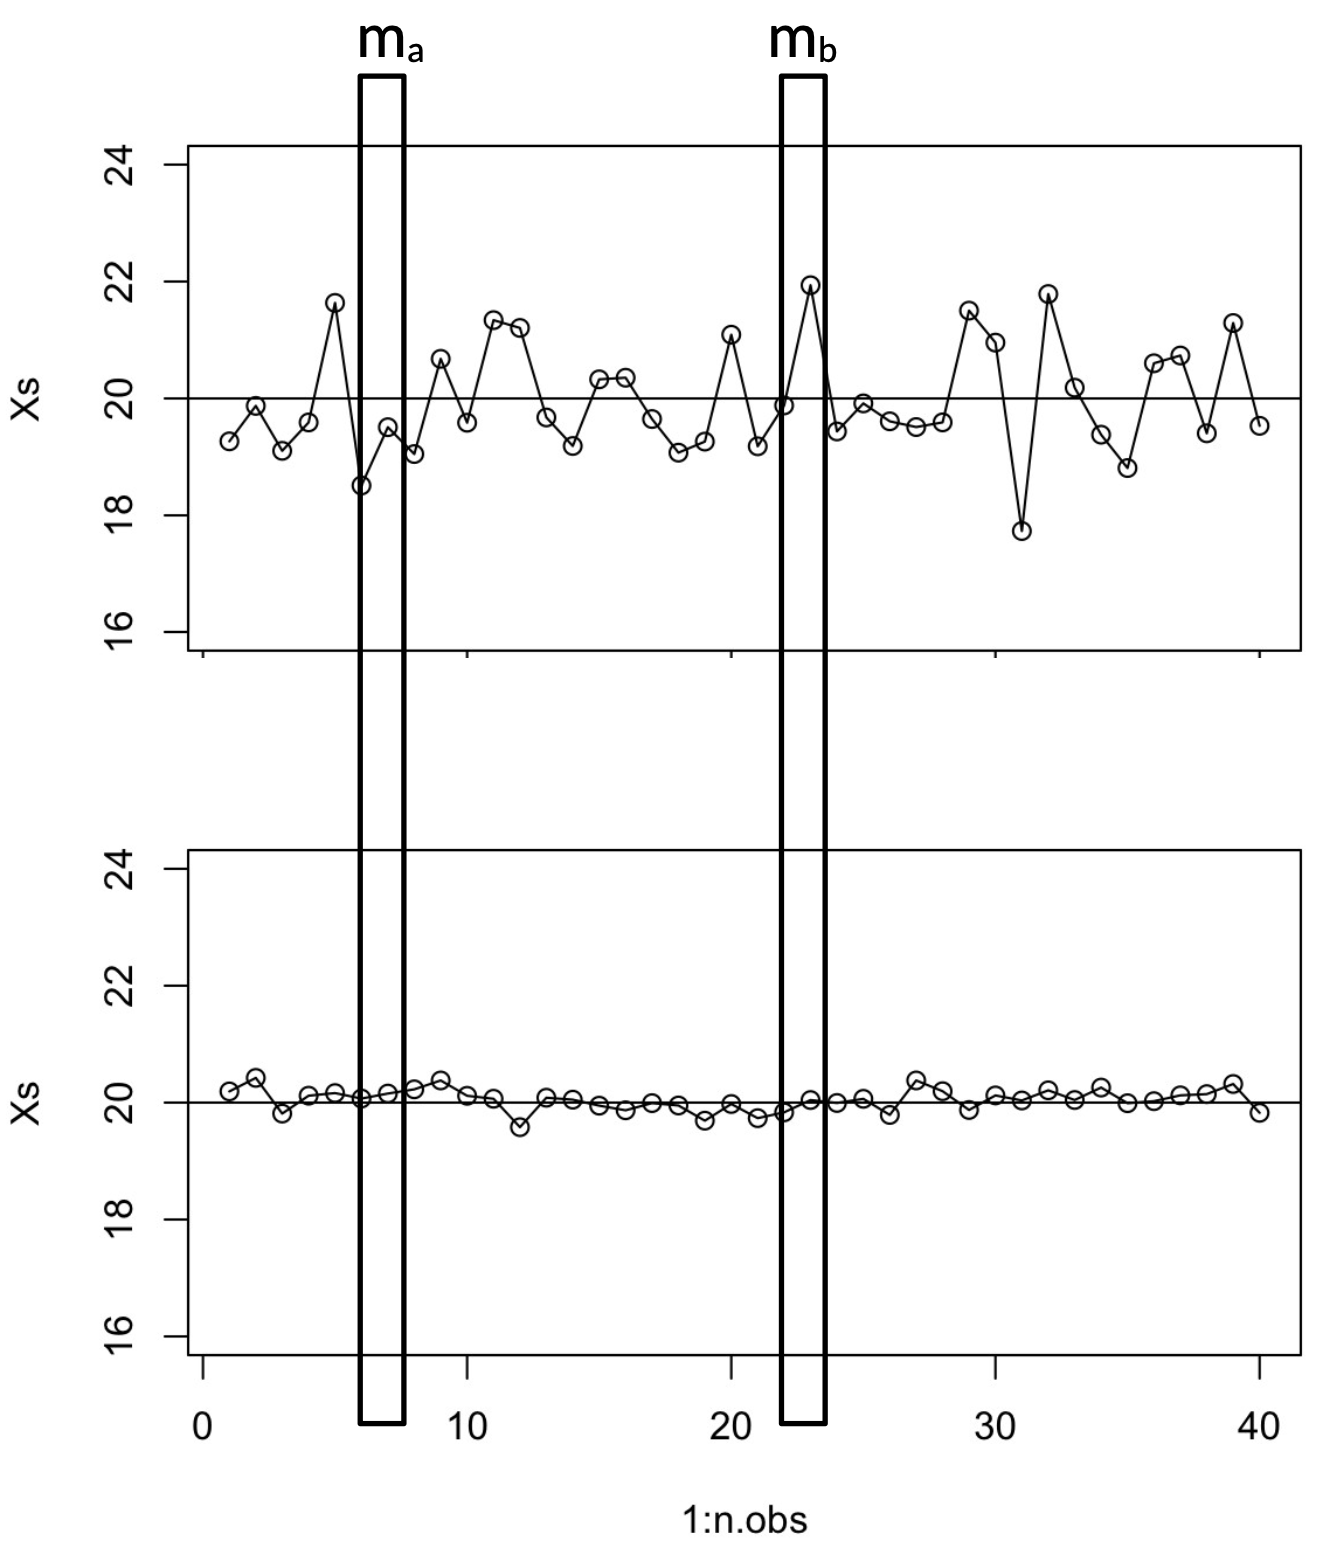
\includegraphics[scale=0.25]{Figures/affidabilità_test_retest.png}
    \end{figure}
  \end{column}
  \begin{column}{0.5\textwidth}
    Test bassa affidabilità test-retest
    
    \vspace{6em}
    Test alta affidabilità test-retest
  \end{column}
\end{columns}
\end{frame}

\begin{frame}{Affidabilità test-retest}
\phantomsection\label{affidabilituxe0-test-retest-4}
Perché viene spesso usato il coefficiente di correlazione di Pearson
(\(r\)) se non è adeguato? \vspace{2em}

Probabilmente per semplice convenzione e per semplicità (il coefficiente
r di pearson può esprimere facilmente la varianza condivisa tra le
variabili, semplicemente calcolando \(r^2\)).

Non è completamente sbagliato e può fornire un quadro abbastanza
completo se accompagnato da t-tests (per indagare differenze
sistematiche).
\end{frame}

\begin{frame}{Affidabilità test-retest}
\phantomsection\label{affidabilituxe0-test-retest-5}
Esistono diversi modi di misurare l'affidabilità test-retest e sempre
più spesso si usano formule più appropriate, in particolare
l'\textbf{Intraclass Correlation (ICC)} basata sull'\emph{accordo
assoluto}, che tiene conto anche degli effetti sistematici (le formule
della ICC saranno trattate per l'inter-rater agreement).

\vspace{1em}

\small

Nel tipico disegno test-retest (due occasioni prestabilite, uguali per
tutti) si raccomanda un modello ICC a due vie, a effetti misti, basato
sull'accordo assoluto e riferito a una singola misurazione --- spesso
indicato come ICC(2,1) o ICC(A,1) (Shrout \& Fleiss, 1979; McGraw \&
Wong, 1996; Koo \& Li, 2016).

\emph{Soglie indicative}: \(\geq 0.70\) per ricerca/confronti tra
gruppi; per decisioni sul singolo individuo spesso \(\geq 0.90\),
idealmente \(\sim 0.95\) (Nunnally \& Bernstein, 1994).
\end{frame}

\section{Inter-rater agreement}\label{inter-rater-agreement}

\begin{frame}{Inter-rater agreement}
\phantomsection\label{inter-rater-agreement-1}
\small

\textbf{Inter-rater agreement} (o \emph{affidabilità inter-rater}):
quanto è consistente il punteggio assegnato da valutatori diversi che
osservano la stessa prestazione. È praticamente per definizione legato
all'\emph{oggettività} del test (l'indipendenza del risultato
dall'osservatore).

È tendenzialmente più basso nei test in cui la risposta non è univoca o
è graduata (es. disegno, descrizione, interpretazione di proverbi), più
alto quando la risposta corretta è univoca e dicotomica (es. digit
span). Al di là della complessità del comportamento, l'elemento cruciale
e trasversale è la \textbf{chiarezza delle regole di attribuzione dei
punteggi}, comprese le indicazioni per i casi ambigui.
\end{frame}

\begin{frame}{Inter-rater agreement}
\phantomsection\label{inter-rater-agreement-2}
\small

La formula più utilizzata è l'\textbf{Intraclass Correlation (ICC)}. A
differenza della correlazione (solo 2 variabili), l'ICC può essere usata
per \(k\) raters.

L'ICC non è un singolo coefficiente ma una \textbf{famiglia} di
coefficienti, che assumono relazioni diverse tra gruppi e osservazioni e
si basano su scomposizione della varianza (ANOVA / mixed-effects). Per
l'inter-rater agreement sono rilevanti le ICC basate
sull'\textbf{accordo assoluto} (valori alti solo se i raters assegnano
più o meno lo stesso punteggio, non solo se i punteggi sono correlati).

\href{https://en.wikipedia.org/wiki/Intraclass_correlation}{\ul{https://en.wikipedia.org/wiki/Intraclass\_correlation}}
\end{frame}

\begin{frame}{Inter-rater agreement}
\phantomsection\label{inter-rater-agreement-3}
\small

Una versione spesso utilizzata è la \textbf{ICC(2,1) agreement}: si
assume che diversi rater vedano la stessa prestazione dello stesso
soggetto e si ottiene una stima dell'agreement in termini assoluti.

\[
ICC(2,1) = \frac{MSB - MSE}
{MSB + (n_j - 1)MSE + \frac{n_j(MSJ - MSE)}{n_c}}
\]

\[
\scriptsize
\begin{aligned}
MSB, MSJ & = \text{varianza tra soggetti, tra giudici (rater)} \\
MSE & = \text{varianza dell'interazione giudici} \times \text{soggetti} \\
n_c, n_j & = \text{numero di giudici, di casi}
\end{aligned}
\]
\end{frame}

\begin{frame}{Inter-rater agreement}
\phantomsection\label{inter-rater-agreement-4}
\begin{columns}
  \begin{column}{0.5\textwidth}
    \begin{figure}
    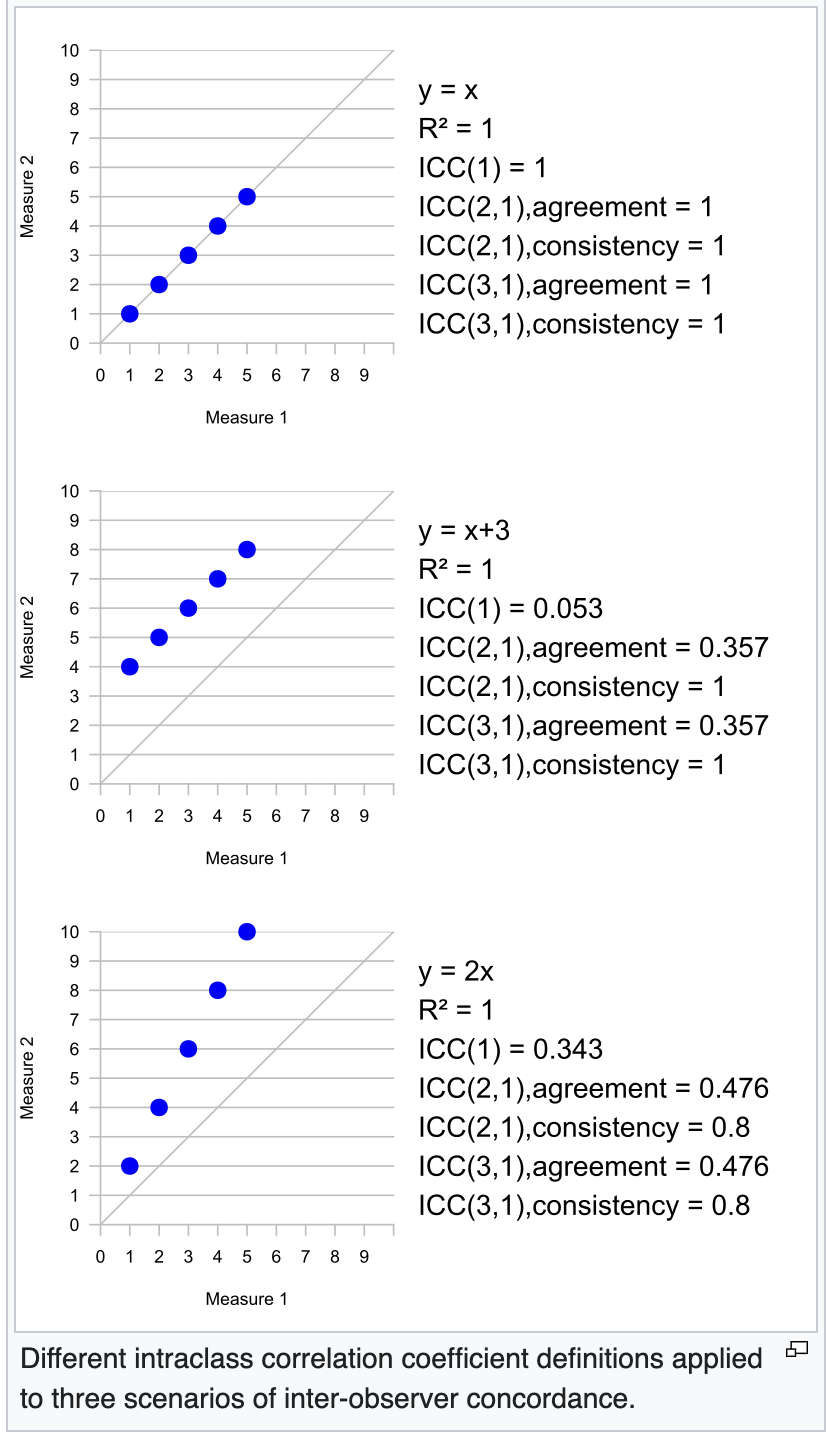
\includegraphics[scale=0.2]{Figures/wiki_ICC.png}
    \end{figure}
    \footnote{Da pagina Wikipedia Intraclass Correlation}
  \end{column}
  \begin{column}{0.5\textwidth}
    La figura mostra come diverse relazioni sono catturate da diversi coefficienti.
    
    Nota che $R^2$ è il coefficiente di correlazione $r$ elevato al quadrato, ma è anche usato nelle regressioni (in breve altre analisi statistiche dove si indaga la relazione tra variabili usando equazione del tipo $y = bx + e$).
  \end{column}
\end{columns}
\end{frame}

\begin{frame}{Alcune considerazioni su ICC}
\phantomsection\label{alcune-considerazioni-su-icc}
\textbf{Perché non è sempre usata ICC anche per test-retest visto che
tiene conto anche di differenze sistematiche?}

Probabilmente per prassi e convenzione (che si osserva soprattutto nei
test in Italiano). In letteratura è però possibile trovare alcuni studi
che la utilizzano anche per test-retest e nel corso degli anni sempre
più autori seguono la più appropriata formula di ICC. In caso di effetto
pratica sarebbe infatti più adeguata.

\vspace{1em}

\small \emph{Soglie indicative} per l'inter-rater agreement (ICC):
\(< 0.40\) scarso, \(0.40 - 0.59\) discreto, \(0.60 - 0.74\) buono,
\(\geq 0.75\) eccellente (Cicchetti \& Sparrow, 1981); con
classificazione simile, Fastenau et al.~(1996) considerano \(0.60\) la
soglia per un accordo ``sostanziale'' e \(0.75 - 0.80\) per uno ``quasi
perfetto''.
\end{frame}

\section{Consistenza interna (e
split-half)}\label{consistenza-interna-e-split-half}

\begin{frame}{Affidabilità split-half}
\phantomsection\label{affidabilituxe0-split-half}
Un approccio tradizionale per calcolare la consistenza degli item di un
test è dividere in due il test (tipicamente item pari da un lato,
dispari dall'altro) e calcolare la correlazione tra i punteggi delle due
metà nei vari partecipanti. \textbf{Questo metodo è detto split-half
reliability (o affidabilità split-half)}.

Poiché ciascuna metà è più corta dell'intero test, la correlazione tra
le due metà \textbf{sottostima} l'affidabilità del test completo: si
applica quindi la correzione di \textbf{Spearman-Brown}.

Limite principale: il risultato dipende, almeno in parte, da come si
divide il test. Per questo si preferisce la sua estensione, la
\emph{consistenza interna}. \emph{Soglia indicativa}:
\(\geq 0.70 - 0.80\) (Slick, 2006).
\end{frame}

\begin{frame}{Consistenza interna}
\phantomsection\label{consistenza-interna}
\textbf{Consistenza interna}: rappresenta quanto gli item di un test
siano tra loro coerenti, cioè quanto misurino (almeno in parte) la
stessa cosa.

Concettualmente stima quale sarebbe la correlazione media considerando
\emph{tutte} le possibili divisioni split-half. È un concetto a cavallo
tra affidabilità e validità (struttura fattoriale del test).
\end{frame}

\begin{frame}{Formula di Kuder-Richardson (K-R 20)}
\phantomsection\label{formula-di-kuder-richardson-k-r-20}
È una formula che viene usata quando gli item sono dicotomici (0/1)

\[
r_{KR20} = \left(\frac{n}{n-1}\right)\frac{s_t^2 - \sum{pq}}{s_t^2}
\]

\[
\small
\begin{aligned}
n & = \text{numero di items nel test} \\
s_t^2 & = \text{varianza del punteggio totale nel test} \\
\sum{pq} & = \text{somma del prodotto $p$ x $q$ in ogni item del test} \\
p & = \text{proporzione delle persone che passano l’item (o risposta 1)} \\
q & = \text{proporzione delle persone che non passano l’item (o risposta 0)}
\end{aligned}
\]
\end{frame}

\begin{frame}{Cronbach's alpha}
\phantomsection\label{cronbachs-alpha}
È l'indice più diffuso, una generalizzazione della formula KR-20 al caso
di item non dicotomici

\[
\alpha = \left(\frac{n}{n-1}\right)\frac{s_t^2 - \sum{s_i^2}}{s_t^2}
\]

\[
\small
\begin{aligned}
n & = \text{numero di items nel test} \\
s_t^2 & = \text{varianza del punteggio totale nel test} \\
s_i^2 & = \text{varianza di ogni item al test} \\
\end{aligned}
\]

\footnotesize \(\alpha\) è un \emph{limite inferiore} dell'affidabilità
e assume item (essenzialmente) tau-equivalenti e unidimensionali.
\end{frame}

\begin{frame}{Altri metodi per calcolare la consistenza interna}
\phantomsection\label{altri-metodi-per-calcolare-la-consistenza-interna}
\small

Sebbene KR-20 e \(\alpha\) siano i più comuni, hanno limiti intrinseci
(es. assumono unidimensionalità).

\begin{itemize}
\tightlist
\item
  \textbf{omega di McDonald (\(\omega\))}: alternativa più recente e
  considerata \textbf{più robusta}, adatta anche in caso di
  multidimensionalità; oggi spesso raccomandata come default.
\item
  \textbf{GLB (Greatest Lower Bound)}: preferibile se i punteggi degli
  item non sono normali.
\end{itemize}

\(\omega\) e GLB sono legati alle analisi fattoriali (vedi slides su
validità) e computazionalmente più complessi. Per i \textbf{test di
velocità} la consistenza interna non è una misura appropriata.

\emph{Soglie indicative}: \(< 0.70\) inaccettabile, \(0.70 - 0.79\)
discreto, \(0.80 - 0.89\) buono, \(\geq 0.90\) eccellente (Slick, 2006);
nei test neuropsicologici spesso \(\sim 0.60\).
\end{frame}

\begin{frame}{Item selection}
\phantomsection\label{item-selection}
\small

Un concetto associato a KR-20, Cronbach's alpha, e altre misure di
consistenza interna è quello dell'item selection e cioè quella procedura
nella creazione di un test di identificazione degli item da mantenere
nel test finale.

Alcune misure sono specifiche per items (un po' come I loadings
nell'analisi fattoriale).

Esempi che vengono dall'alpha di Cronbach:

\begin{itemize}
\item
  \textbf{r-drop}: indica la correlazione tra il test, e il test tolto
  quell'item (si ha dunque un valore r-drop per item)
\item
  \textbf{r-cor}: indica la correlazione tra l'item e il test totale
  controllando per overlap con altri item e per affidabilità globale.
\end{itemize}
\end{frame}

\begin{frame}{Interpretare l'affidabilità a livello del test}
\phantomsection\label{interpretare-laffidabilituxe0-a-livello-del-test}
\small

Ogni sorgente di affidabilità può essere usata per stimare l'errore di
misura del test.

Il coefficiente di affidabilità (indipendente dalla formula) può infatti
essere interpretato come la percentuale di variabilità riconducibile al
punteggio vero, trasformando semplicemente il coefficiente in
percentuale. Questo segue la definizione che viene fatta a priori di
cosa è l'affidabilità.

Ad esempio:

Una correlazione test-retest 0.8 vuol dire che l'80\% di variabilità
test-retest è riconducibile alla variabilità del punteggio vero.

Una consistenza interna di 0.9 vuol dire che il 90\% di variabilità
nella consistenza interna è riconducibile alla variabilità del punteggio
vero, etc.
\end{frame}

\begin{frame}{Interpretare l'affidabilità a livello del test}
\phantomsection\label{interpretare-laffidabilituxe0-a-livello-del-test-1}
L'errore associato ad ogni sorgente di affidabilità è pertanto
calcolabile come:

\[
Errore = (1-C_a) \times 100
\] Dove \(C_a\) è il coefficiente di affidabilità in questione (es.
Affidabilità test retest, affidabilità inter rater, etc).
\end{frame}

\begin{frame}{Combinare diversi tipi di errore}
\phantomsection\label{combinare-diversi-tipi-di-errore}
Calcolando diverse sorgenti di errore è possibile sommarle (assumendo la
loro indipendenza) per ottenere un errore totale e calcolare quindi la
variabilità del punteggio che si presume sia riconducibile al punteggio
vero

Es. supponiamo di avere un test che ha le seguenti caratteristiche:

\begin{itemize}
\tightlist
\item
  Affidabilità test-retest = 0.85 (\(r\) di pearson)
\item
  Affidabilità inter-rater = 0.70 (\(ICC(2,1)\))
\item
  Consistenza interna = 0.97 (alpha di Cronbach)
\end{itemize}
\end{frame}

\begin{frame}{Combinare diversi tipi di errore}
\phantomsection\label{combinare-diversi-tipi-di-errore-1}
Errore test-retest: \((1-0.85) \times 100 = 15\%\)

Errore inter-rater: \((1-0.7) \times 100 = 30\%\)

Errore consistenza interna: \((1-0.97) \times 100 = 3\%\)

Errore totale: \(15 + 30 + 3 = 48\%\) \vspace{1em}

A livello di test il 48\% della varianza è riconducibile ad errore, e il
52\% (100 -- 48) al punteggio vero (che è anche l'affidabilità
complessiva del test). (Vedi Urbina, 2004, per un esempio simile)

\vspace{0.5em}

\footnotesize \textbf{Attenzione}: questa scomposizione additiva assume
che le sorgenti di errore siano \emph{indipendenti} ed è un artificio
grossolano. Nella pratica psicometrica la precisione complessiva è
espressa più propriamente tramite l'errore standard di misurazione
(\emph{SEM}) e i relativi intervalli di confidenza (non approfonditi
qui).
\end{frame}

\begin{frame}{Stimare il punteggio vero}
\phantomsection\label{stimare-il-punteggio-vero}
Le formule di affidabilità ci permettono inoltre di stimare il punteggio
vero

\[
T'=r_{xx}(X-M)+M
\] \[
\small
\begin{aligned}
T' & = \text{stima del punteggio vero} \\
r_{xx} & = \text{affidabilità complessiva (vedi slide precedente)} \\
X & = \text{punteggio osservato} \\
M & = \text{media del campione di riferimento} \\
\end{aligned}
\]
\end{frame}

\begin{frame}{Stimare il punteggio vero: alcune note}
\phantomsection\label{stimare-il-punteggio-vero-alcune-note}
\begin{enumerate}
[1)]
\tightlist
\item
  La stima del punteggio vero è spesso accompagnata anche dalla
  creazione di intervalli di confidenza attorno alla stima (riprenderemo
  questo quando parleremo di cut-offs, vedi anche Appendice)
\end{enumerate}
\end{frame}

\begin{frame}{Affidabilità ed errore}
\phantomsection\label{affidabilituxe0-ed-errore}
Nota che nell'approccio prima descritto (di stimare l'affidabilità
globale a partire dalle diverse affidabilità), più informazioni abbiamo
più bassa sarà la percentuale riconducibile alla varianza del punteggio
vero.

Un altro modo per pensare il problema è che stimare la varianza
riconducibile a punteggio vero a partire da un solo indice sarà
inevitabilmente una sovrastima della stessa.
\end{frame}

\begin{frame}{Affidabilità ed errore}
\phantomsection\label{affidabilituxe0-ed-errore-1}
\begin{center}
  \textbf{Stimare il punteggio vero: alcune note}
\end{center}

\small

\begin{enumerate}
[1)]
\setcounter{enumi}{1}
\tightlist
\item
  Per stimare il punteggio vero entra due volte in gioco la media del
  campione di riferimento (denotata con M). Questo permette di tenere in
  considerazione un fenomeno detto \textbf{regressione verso la media}:
  in ogni misura con errore è sempre più probabile che una misura
  successiva sia più vicina alla media del campione di riferimento.
  Questo perché, specie se l'errore dello strumento è grande, ogni
  deviazione della media ha probabilità di essere dovuta al caso.
\end{enumerate}

Correggere per la media ha però un grosso limite intrinseco: con che
media correggere? Ad esempio, se ho un paziente con TBI è corretto usare
(per M), la media del gruppo di sani con cui è stato sviluppato il test?
\end{frame}

\begin{frame}{Stimare il punteggio vero: alcune note}
\phantomsection\label{stimare-il-punteggio-vero-alcune-note-1}
Questo tipo di limiti rende complessa l'applicazione di formule per
stimare il punteggio vero. Vedremo in futuro comunque in utilizzi
clinici e pratici (es. cut-off, valori di cambiamento), \textbf{quasi
sempre non sono usati i punteggi veri ma i punteggi osservati}.
\end{frame}

\begin{frame}{Come considerare i coefficienti di affidabilità}
\phantomsection\label{come-considerare-i-coefficienti-di-affidabilituxe0}
Ogni coefficiente di affidabilità, in generale, stima la varianza
riconducibile al punteggio vero rispetto alla variabilità totale (cioè
quella che si rileva nei punteggi osservati), utilizzando diverse
formule (es. \(r\) di Pearson, \(ICC(2,1)\), etc.).

L'idea generale può essere espressa da questa formula.

\[
r_{xx} = \frac{\sigma_{true}}{\sigma_{tot}}
\]
\end{frame}

\section{Riferimenti}\label{riferimenti}

\begin{frame}{Riferimenti}
\phantomsection\label{riferimenti-1}
\footnotesize

\begin{itemize}
\tightlist
\item
  AERA, APA, \& NCME (2014). \emph{Standards for Educational and
  Psychological Testing}.
\item
  Cicchetti, D. V., \& Sparrow, S. A. (1981). \emph{American Journal of
  Mental Deficiency}.
\item
  Fastenau, P. S., et al.~(1996).
\item
  Koo, T. K., \& Li, M. Y. (2016). \emph{Journal of Chiropractic
  Medicine}.
\item
  McGraw, K. O., \& Wong, S. P. (1996). \emph{Psychological Methods}.
\item
  Nunnally, J. C., \& Bernstein, I. H. (1994). \emph{Psychometric
  Theory} (3rd ed.).
\item
  Sattler, J. M. (2001). \emph{Assessment of Children}.
\item
  Shrout, P. E., \& Fleiss, J. L. (1979). \emph{Psychological Bulletin}.
\item
  Slick, D. J. (2006). Psychometrics in neuropsychological assessment.
  In Spreen \& Strauss (cap. 1).
\item
  Urbina, S. (2004). \emph{Essentials of Psychological Testing}.
\end{itemize}
\end{frame}




\end{document}
